\documentclass[8pt,a4paper,compress]{beamer}

\usepackage{/home/siyer/lib/slides}

\title{Substring Search}
\date{}
\begin{document}
\begin{frame}
\vfill
\titlepage
\end{frame}

\begin{frame}
\frametitle{Outline}
\tableofcontents
\end{frame}

\section{Substring Search}
\begin{frame}[fragile]
\pause

A fundamental operation on strings is substring search: given a text string of length $N$ and a pattern string of length $M$, find an occurrence of the pattern within the text, as in the following example

\begin{center}
\visible<2->{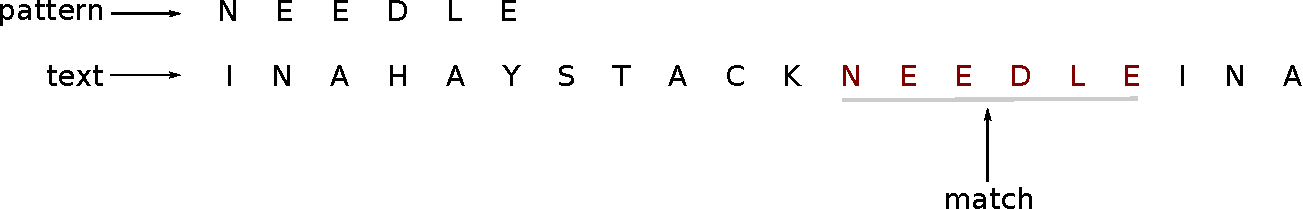
\includegraphics[scale=0.4]{figures/subsearch1.pdf}}
\end{center}

\pause
\bigskip

Most algorithms for this problem can easily be extended to find all occurrences of the pattern in the text, to count the number of occurrences of the pattern in the text, or to provide context (substrings of the text surrounding each occurrence of the pattern)

\pause
\bigskip

To best appreciate the algorithms, think of the pattern as being relatively short (with $M$ equal to, say, 100 or 1,000) and the text as being relatively long (with $N$ equal to, say, 1 million or 1 billion)

\pause
\bigskip

In substring search, we typically preprocess the pattern in order to be able to support fast searches for that pattern in the text
\end{frame}

\section{Brute-force Substring Search}
\begin{frame}[fragile]
\pause

An obvious method for substring search is to check, for each possible position in the text at which the pattern could match, whether it does in fact match

\pause
\bigskip

The \lstinline{search()} method below implements this idea
\begin{lstlisting}[language=Java]
public static int search(String pat, String txt) {
    int M = pat.length();
    int N = txt.length();
    for (int i = 0; i <= N - M; i++) {
        int j;
        for (j = 0; j < M; j++) {
            if (txt.charAt(i + j) != pat.charAt(j)) {
                break;
            }
        }
        if (j == M) { 
            return i; // found
        } 
    }
    return N;         // not found
}
\end{lstlisting}
\end{frame}

\begin{frame}[fragile]
\pause

Trace
\begin{center}
\visible<2->{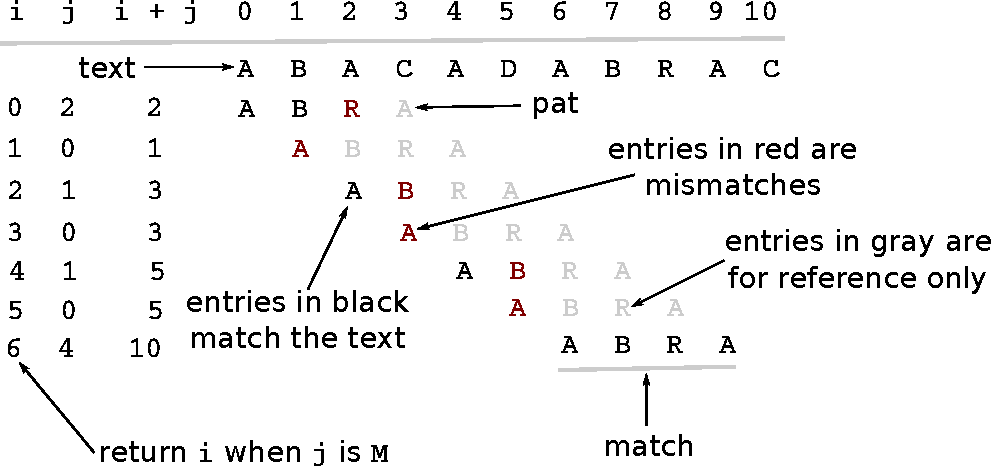
\includegraphics[scale=0.45]{figures/subsearch2.pdf}}
\end{center}

\pause
\bigskip

Brute-force substring search requires $\sim NM$ character compares to search for a pattern of length $M$ in a text of length $N$, in the worst case
\end{frame}

\begin{frame}[fragile]
\pause

Alternate implementation of brute-force substring search (explicit backup)

\begin{lstlisting}[language=Java]
public static int search(String pat, String txt) {
    int j, M = pat.length();
    int i, N = txt.length();
    for (i = 0, j = 0; i < N && j < M; i++) {
        if (txt.charAt(i) == pat.charAt(j)) { 
            j++; 
        }
        else { 
            i -= j; 
            j = 0; 
        }
    }
    if (j == M) { 
        return i - M;  // found
    }
    return N;          // not found 
}
\end{lstlisting}
\end{frame}

\section{Knuth-Morris-Pratt (KMP) Substring Search}
\begin{frame}[fragile]
\pause

Basic idea: whenever we detect a mismatch, we already know some of the characters in the text (since they matched the pattern characters
prior to the mismatch), so we can avoid backing up the text pointer over all those known characters

\pause
\bigskip

For example
\begin{center}
\visible<3->{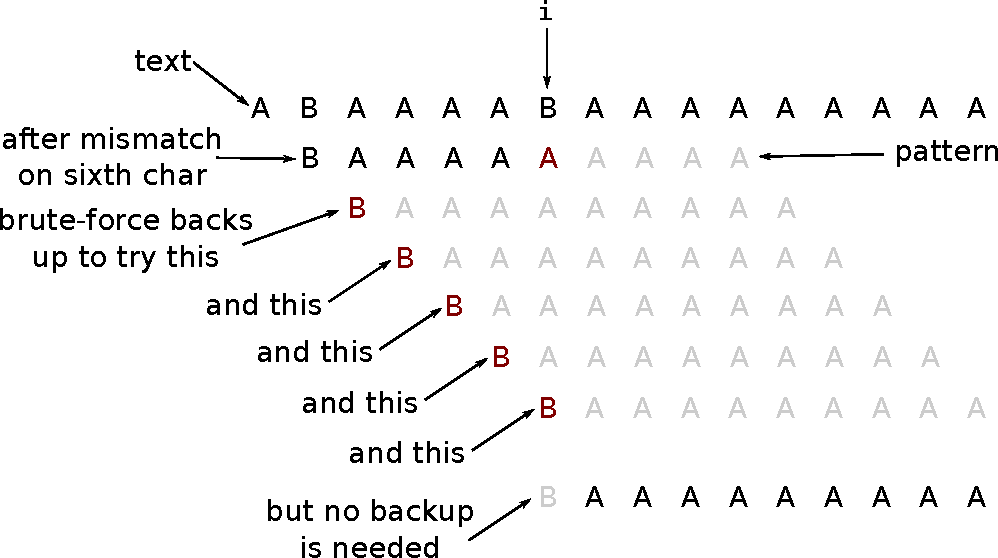
\includegraphics[scale=0.45]{figures/subsearch3.pdf}}
\end{center}
\end{frame}

\begin{frame}[fragile]
\pause

In KMP substring search, we never back up the text pointer \lstinline{i}, and we use an array \lstinline{dfa[][]} (DFA stands for deterministic finite-state automaton) to record how
far to back up the pattern pointer \lstinline{j} when a mismatch is detected

\pause
\bigskip

For every character \lstinline{c}, \lstinline{dfa[c][j]} is the pattern position to compare against the next text position after comparing \lstinline{c} with \lstinline{pat.charAt(j)}

\pause
\bigskip

During the search, \lstinline{dfa[txt.charAt(i)][j]} is the pattern position to compare with \lstinline{txt.charAt(i + 1)} after comparing \lstinline{txt.charAt(i)} with \lstinline{pat.charAt(j)}

\pause
\bigskip

KMP substring search (DFA simulation)
\begin{lstlisting}[language=Java]
public int search(String txt) { 
    int M = pat.length();
    int N = txt.length();
    int i, j;
    for (i = 0, j = 0; i < N && j < M; i++) {
        j = dfa[txt.charAt(i)][j];
    }
    if (j == M) { 
        return i - M; // found
    }
    return N;         // not found
}
\end{lstlisting}
\end{frame}

\begin{frame}[fragile]
\pause

DFA corresponding to the pattern \lstinline{A B A B A C}
\begin{center}
\visible<2->{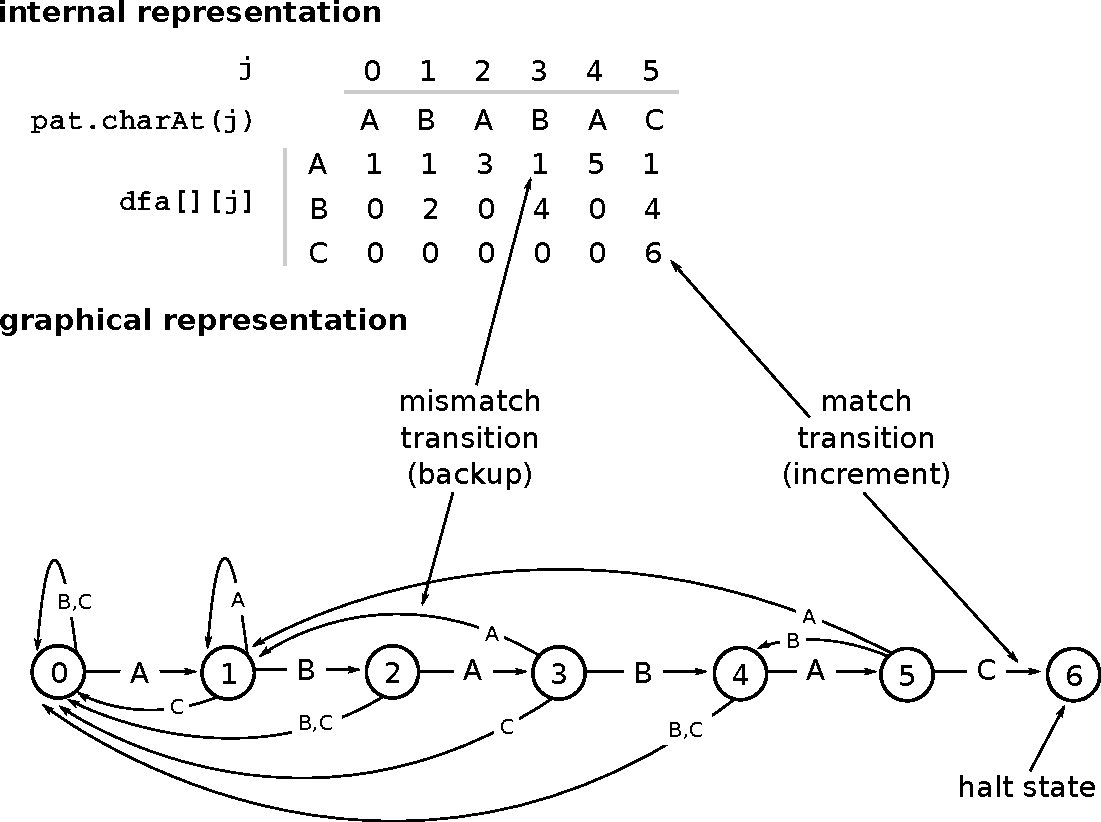
\includegraphics[scale=0.45]{figures/subsearch4.pdf}}
\end{center}
\end{frame}

\begin{frame}[fragile]
\pause

Constructing the DFA: the key observation is that the characters in the text that would need to be rescanned are precisely \lstinline{pat.charAt(1)} through \lstinline{pat.charAt(j - 1)} --- we drop the first character to shift right one position and the last character because of the mismatch

\pause
\bigskip

For each \lstinline{j}
\begin{itemize}
\item Copy \lstinline{dfa[][X] to dfa[][j]} (for mismatch cases)
\item Set \lstinline{dfa[pat.charAt(j)][j]} to \lstinline{j + 1} (for the match case)
\item Update \lstinline{X}
\end{itemize}

\begin{lstlisting}[language=Java]
    dfa = new int[R][M];     
    dfa[pat.charAt(0)][0] = 1; 
    for (int X = 0, j = 1; j < M; j++) {
        for (int c = 0; c < R; c++) { 
            dfa[c][j] = dfa[c][X]; 
        }
        dfa[pat.charAt(j)][j] = j + 1;  
        X = dfa[pat.charAt(j)][X];  
    } 
\end{lstlisting}
\end{frame}

\begin{frame}[fragile]
\pause

Constructing the DFA for KMP substring search for the pattern \lstinline{A B A B A C}
\begin{center}
\visible<2->{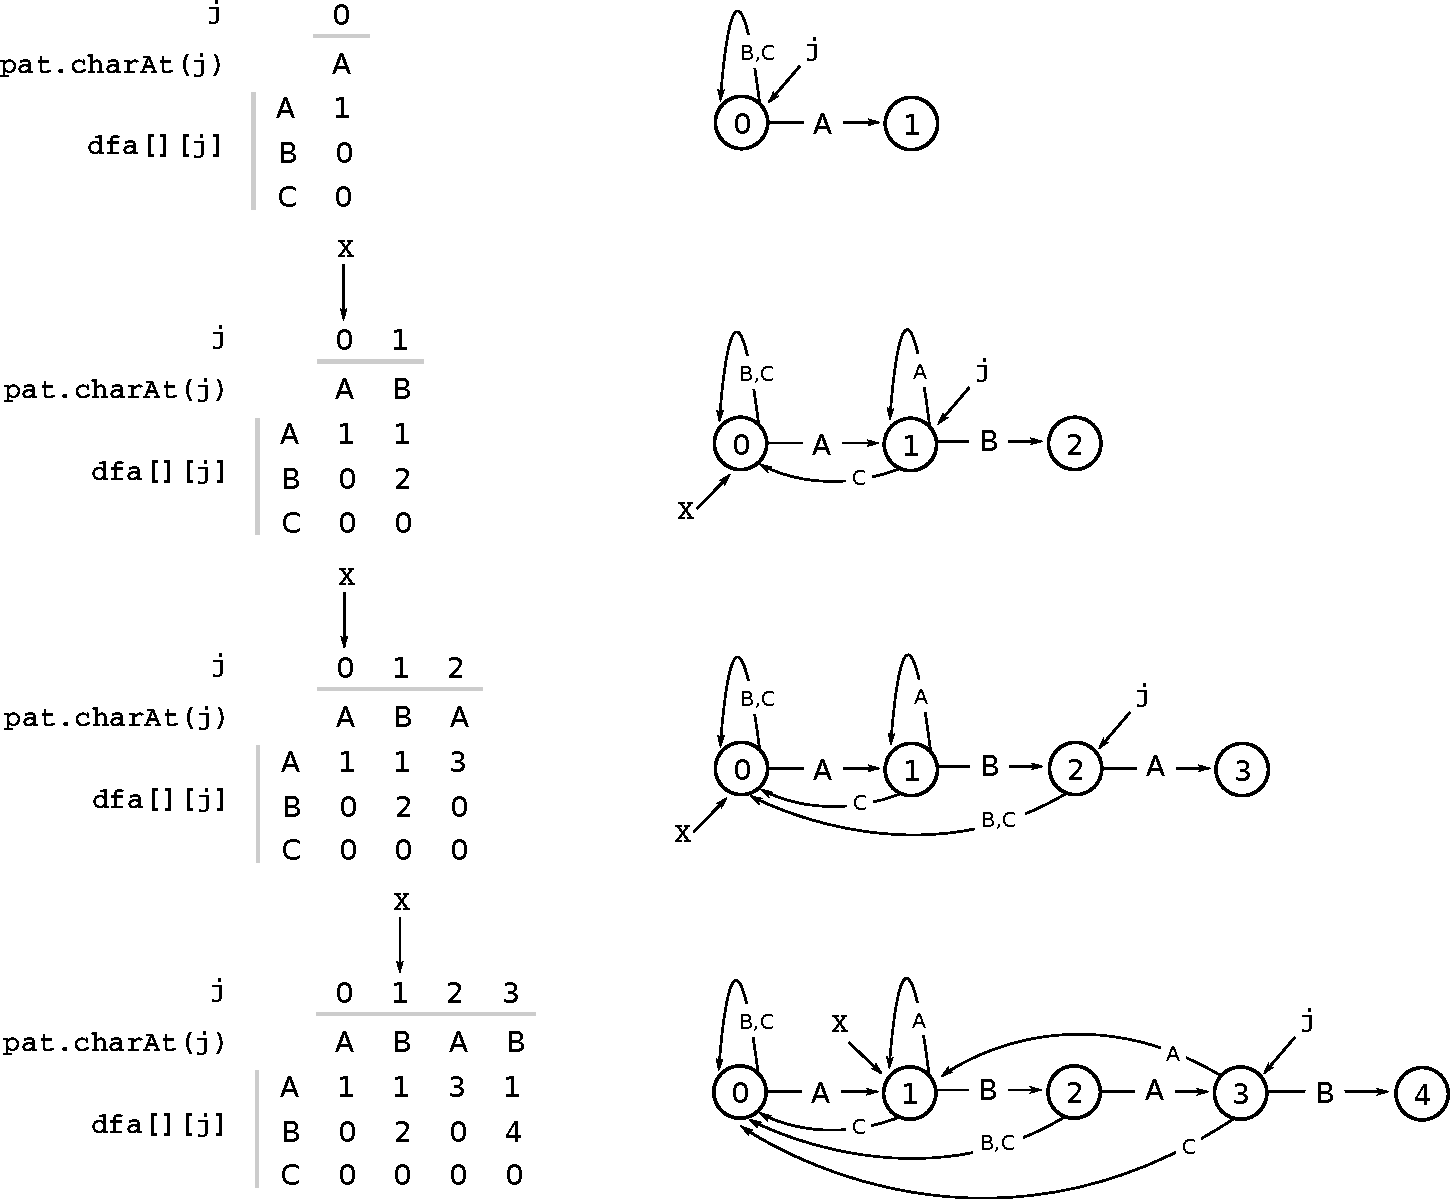
\includegraphics[scale=0.37]{figures/subsearch5.pdf}}
\end{center}
\end{frame}

\begin{frame}[fragile]
\pause

\begin{center}
\visible<2->{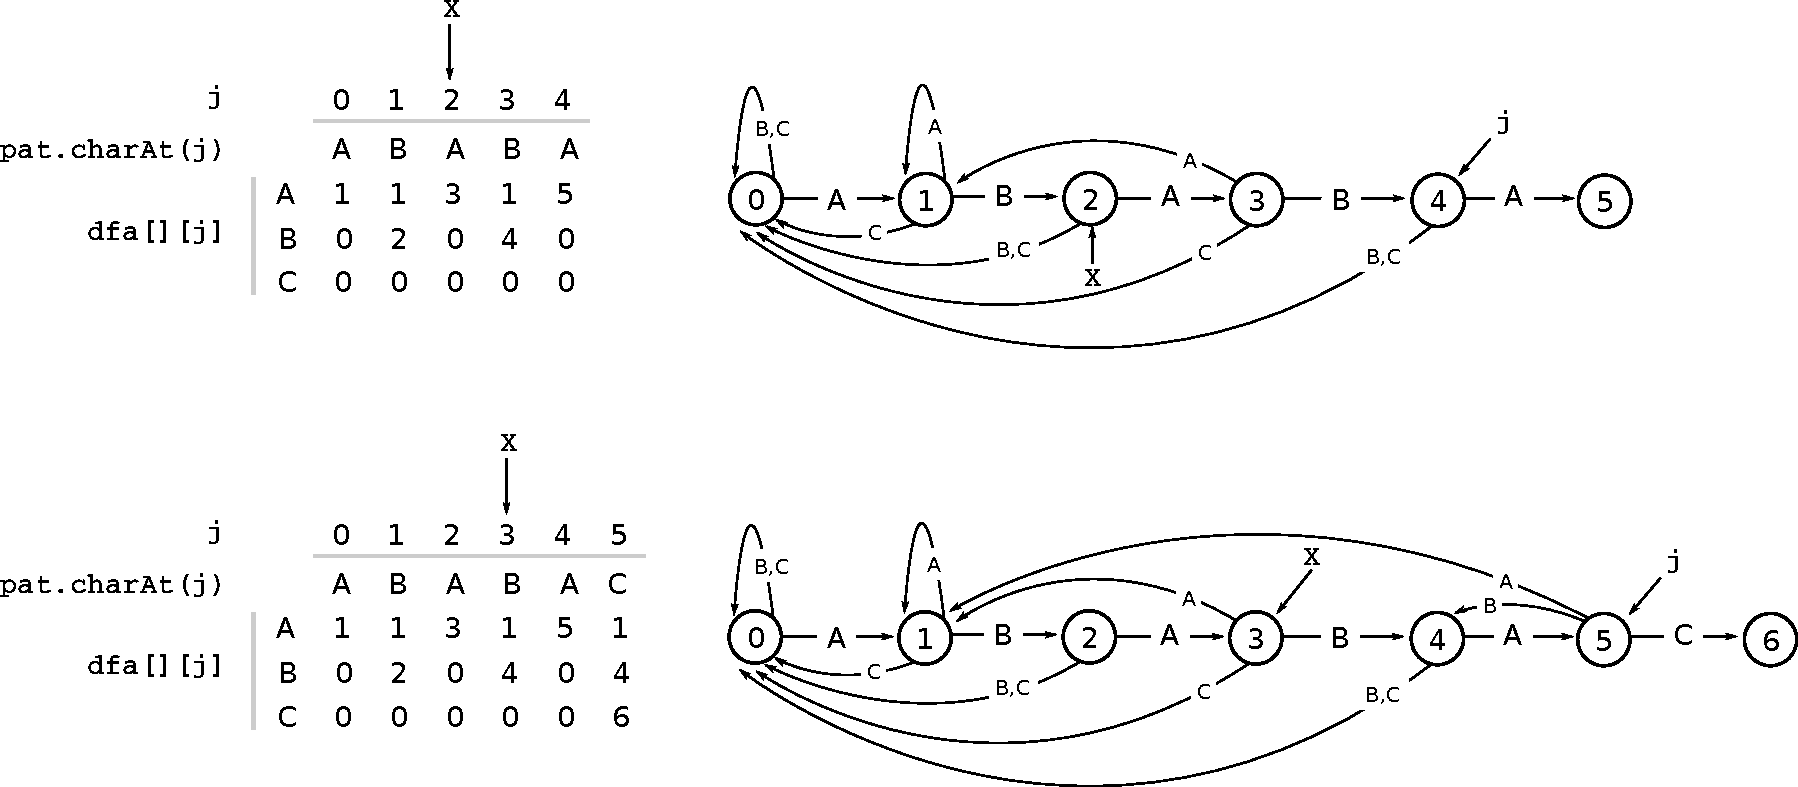
\includegraphics[scale=0.37]{figures/subsearch6.pdf}}
\end{center}
\end{frame}

\begin{frame}[fragile]
\pause

\begin{lstlisting}[language=Java]
package edu.princeton.cs.algs4;

public class KMP {
    private final int R;
    private int[][] dfa;
    private char[] pattern;
    private String pat;

    public KMP(String pat) {
        this.R = 256;
        this.pat = pat;
        int M = pat.length();
        dfa = new int[R][M]; 
        dfa[pat.charAt(0)][0] = 1; 
        for (int X = 0, j = 1; j < M; j++) {
            for (int c = 0; c < R; c++) { dfa[c][j] = dfa[c][X]; }
            dfa[pat.charAt(j)][j] = j + 1;  
            X = dfa[pat.charAt(j)][X];  
        } 
    } 

    public KMP(char[] pattern, int R) {
        this.R = R;
        this.pattern = new char[pattern.length];
        for (int j = 0; j < pattern.length; 
             j++) { this.pattern[j] = pattern[j]; }
        int M = pattern.length;
        dfa = new int[R][M]; 
        dfa[pattern[0]][0] = 1; 
        for (int X = 0, j = 1; j < M; j++) {
            for (int c = 0; c < R; c++) { dfa[c][j] = dfa[c][X]; } 
            dfa[pattern[j]][j] = j + 1; 
            X = dfa[pattern[j]][X];
        } 
    } 
\end{lstlisting}
\end{frame}

\begin{frame}[fragile]
\pause

\begin{lstlisting}[language=Java]
    public int search(String txt) {
        int M = pat.length();
        int N = txt.length();
        int i, j;
        for (i = 0, j = 0; i < N && j < M; i++) { j = dfa[txt.charAt(i)][j]; }
        if (j == M) { return i - M; }
        return N; 
    }

    public int search(char[] text) {
        int M = pattern.length;
        int N = text.length;
        int i, j;
        for (i = 0, j = 0; i < N && j < M; i++) { j = dfa[text[i]][j]; }
        if (j == M) { return i - M; }
        return N;
    }

    public static void main(String[] args) {
        String pat = args[0], txt = args[1];
        char[] pattern = pat.toCharArray();
        char[] text    = txt.toCharArray();
        KMP kmp1 = new KMP(pat);
        int offset1 = kmp1.search(txt);
        KMP kmp2 = new KMP(pattern, 256);
        int offset2 = kmp2.search(text);
        StdOut.println("text:    " + txt);
        StdOut.print("pattern: ");
        for (int i = 0; i < offset1; i++) { StdOut.print(" "); }
        StdOut.println(pat);
        StdOut.print("pattern: ");
        for (int i = 0; i < offset2; i++) { StdOut.print(" "); }
        StdOut.println(pat);
    }
}
\end{lstlisting}
\end{frame}

\begin{frame}[fragile]
\pause

\begin{lstlisting}[language={}]
$ java edu.princeton.cs.algs4.KMP abracadabra abacadabrabracabracadabrabrabracad
text:    abacadabrabracabracadabrabrabracad
pattern:               abracadabra
pattern:               abracadabra
$ java edu.princeton.cs.algs4.KMP rab abacadabrabracabracadabrabrabracad
text:    abacadabrabracabracadabrabrabracad
pattern:         rab
pattern:         rab
$ java edu.princeton.cs.algs4.KMP bcara abacadabrabracabracadabrabrabracad
text:    abacadabrabracabracadabrabrabracad
pattern:                                   bcara
pattern:                                   bcara
$ java edu.princeton.cs.algs4.KMP rabrabracad abacadabrabracabracadabrabrabracad
text:    abacadabrabracabracadabrabrabracad
pattern:                        rabrabracad
pattern:                        rabrabracad
$ java edu.princeton.cs.algs4.KMP abacad abacadabrabracabracadabrabrabracad
text:    abacadabrabracabracadabrabrabracad
pattern: abacad
pattern: abacad
\end{lstlisting}

\pause
\bigskip

Knuth-Morris-Pratt substring search accesses no more than $M + N$ characters to search for a pattern of length $M$ in a text of length $N$
\end{frame}

\section{Performance Characteristics of Substring Search Algorithms}
\begin{frame}[fragile]
\pause

\begin{center}
\begin{tabular}{cccccc}
algorithm & \makecell{operation count \\ guarantee} & \makecell{operation count \\ typical} & \makecell{backup \\ in input?} & correct? & \makecell{extra \\ space} \\ \hline
brute force & $MN$ & $1.1N$ & yes & yes & 1 \\
\makecell{Knuth-Morris-\\Pratt} & $2N$ & $1.1N$ & no & yes & $MR$ \\
Boyer-Moore & $MN$ & $N/M$ & yes & yes & $R$ \\
Rabin-Karp$^\dagger$ & $7N$ & $7N$ & no & yes$^\dagger$ & 1
\end{tabular}

\bigskip

$\dagger$ probabilistic guarantee, with uniform and independent hash function
\end{center}
\end{frame}
\end{document}
